Pour permettre au joueur de contrôler le robot ainsi que le déroulement de la partie, nous avons codé une application pour smartphone Android qui communique les ordres à la carte Arduino via Bluetooth. Dans une 1ère partie nous verrons comment l'application permet au joueur de gérer les différentes phases de jeu au travers de l'interface graphique, puis le code sera expliqué dans une seconde partie.

\section{Description de l'interface graphique}

\label{andr_gui}

\graphicspath{{rc/images/android/}}

L’aspect essentiel de l’application, celui visible par l’utilisateur final et qui lui permettra de juger de sa qualité, est l’interface graphique, appelée aussi GUI (Graphic User Interface). Elle est ici composée de six "vues", défilants les unes après les autres et représentant chacune une étape de la partie entamée par le joueur ; chaque vue est décrite dans un fichier de type XML, utilisant des propriétés propres à Android. \\
La première vue - fig.~\ref{view_0} -, affichée dès le lancement du programme, est très simple et se contente d’afficher un champ textuel indiquant l’état actuel de la connexion entre l’appareil et la carte Arduino. Si la tentative de connexion effectuée automatiquement au démarrage réussit, le message "Connexion en cours..." est remplacé par la vue suivante ; sinon, le message d’erreur "Connexion échouée" est affiché et un bouton "Réessayer" apparaît - fig.~\ref{view_1} - pour permettre à l’utilisateur de redémarrer le processus de connexion après avoir résolu le problème initial, qui bug exclus ne devrait être que l’oubli de l’allumage du robot. \\
La deuxième vue - fig.~\ref{view_2} - propose au joueur de sélectionner entre les différents niveaux de difficulté (voir section~\ref{reg_dif}) ; le joueur choisit aussi le nombre de manches dans la partie (3 par défaut). Lorsqu’il est prêt à lancer la partie, il appuie sur le bouton prévu à cet effet, affichant ainsi la troisième vue. \\
La troisième vue - fig.~\ref{view_3} - demande au joueur le score qu’il a effectué ; elle sera réaffichée à chaque manche de la partie. Lorsque le joueur est prêt, il peut appuyer sur le bouton "J’ai joué !" pour afficher la prochaine vue. \\
La quatrième vue - fig.~\ref{view_4} - est comme la première une vue d’attente où seul le message "Veuillez patienter..." est affiché pendant que le robot, ayant reçu l’ordre du smartphone Android, prépare son tir. L’opération terminée, la carte Arduino indique à l’application qu’elle est prête à tirer : la cinquième vue s’affiche. \\
La cinquième vue - fig.~\ref{view_5} - se compose d’un seul élément intéractif : un bouton qui, lorsqu’appuyé, envoie l’ordre de tirer à la carte Arduino. On y trouve aussi un message de sécurité qui avertit l’utilisateur des risques de passer devant le robot lorsqu’il tire. Le processus recommence à partir de la 3ème vue autant de fois qu’il y a de manches dans la partie, puis s’affiche la dernière vue. \\
La sixième vue - fig.~\ref{view_6} - établit un récapitulatif des scores de tous les joueurs et du robot et indique qui est le vainqueur de la partie. L’utilisateur a ensuite deux possibilités : recommencer une partie et ainsi revenir à la deuxième vue en cliquant sur le bouton prévu à cet effet, ou cliquer sur le bouton "Quitter" pour interrompre l’application.

\begin{figure}

	\begin{minipage}{0.45\textwidth}
		\caption{Connexion en cours}
		\label{view_0}
		\center
		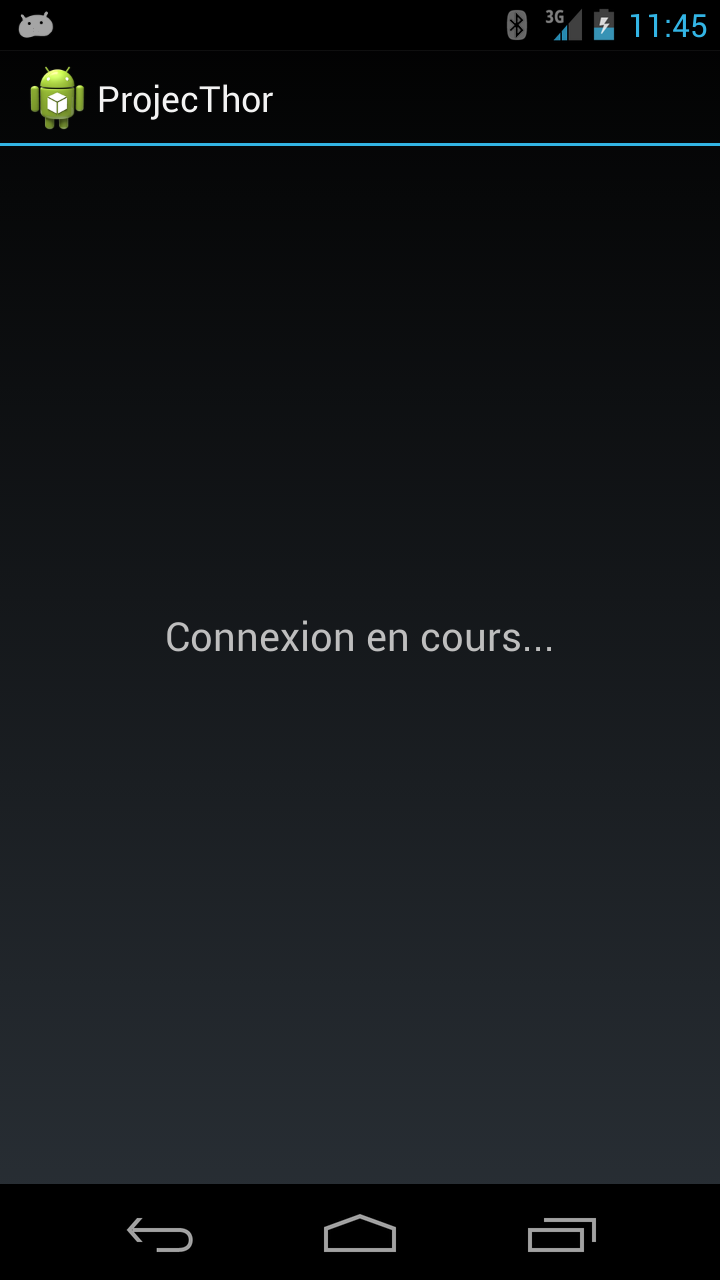
\includegraphics[scale=0.2]{view_1.png}
	\end{minipage}
	\hspace{0.1\textwidth}
	\begin{minipage}{0.45\textwidth}
		\caption{Connexion échouée}
		\label{view_1}
		\center
		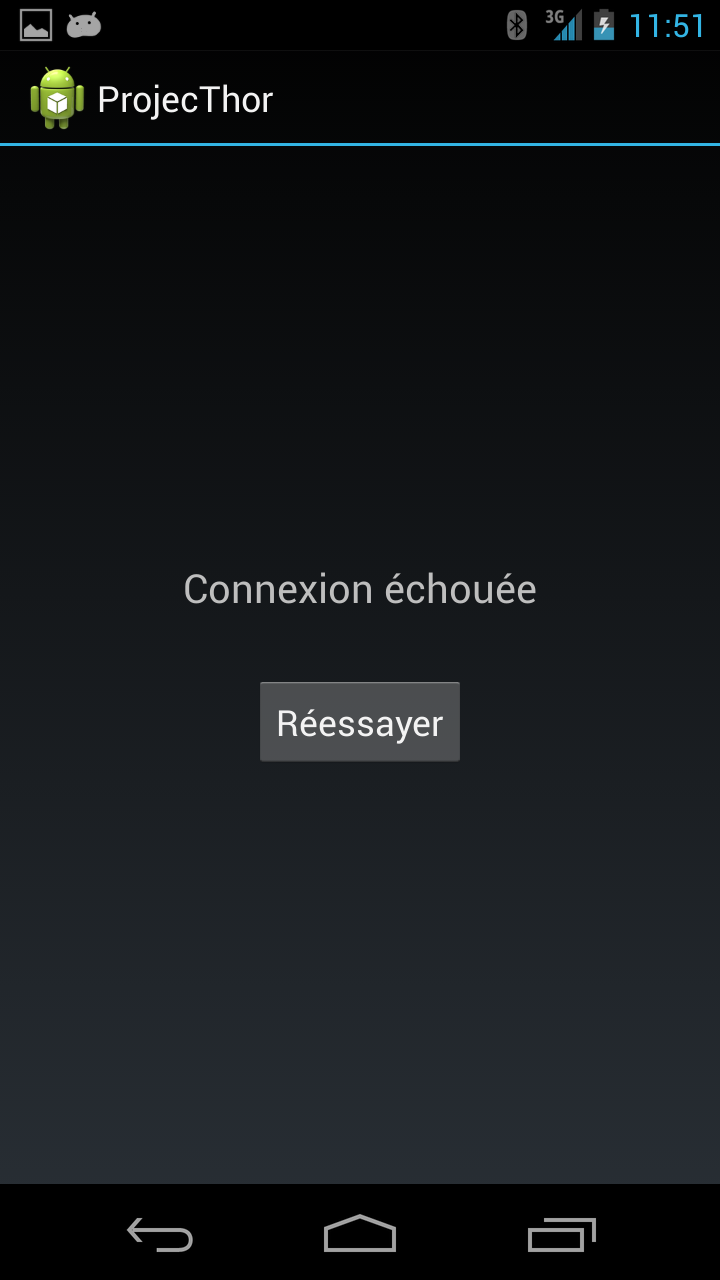
\includegraphics[scale=0.2]{view_0.png}
	\end{minipage}
	
	\vspace*{20mm}

	\begin{minipage}{0.45\textwidth}
		\caption{Réglages avant le lancement de la partie}
		\label{view_2}
		\center
		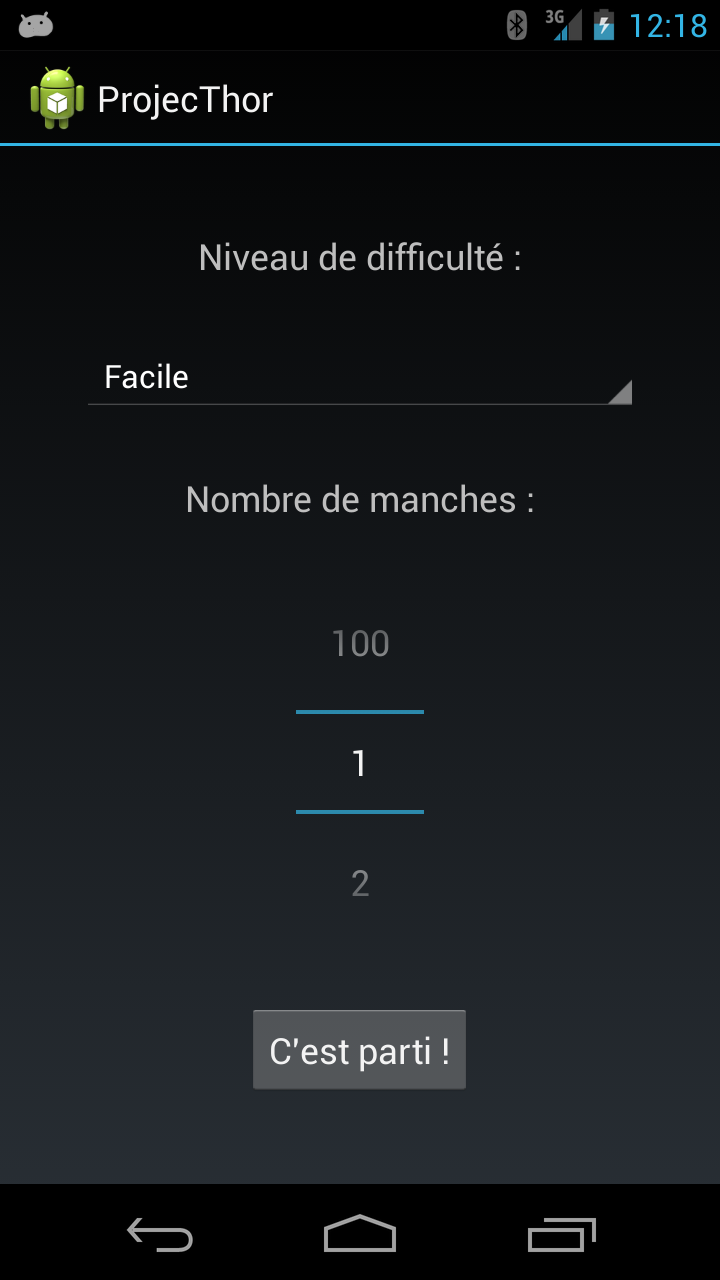
\includegraphics[scale=0.2]{view_2.png}
	\end{minipage}
	\hspace{0.1\textwidth}
	\begin{minipage}{0.45\textwidth}
		\caption{Score du joueur}
		\label{view_3}
		\center
		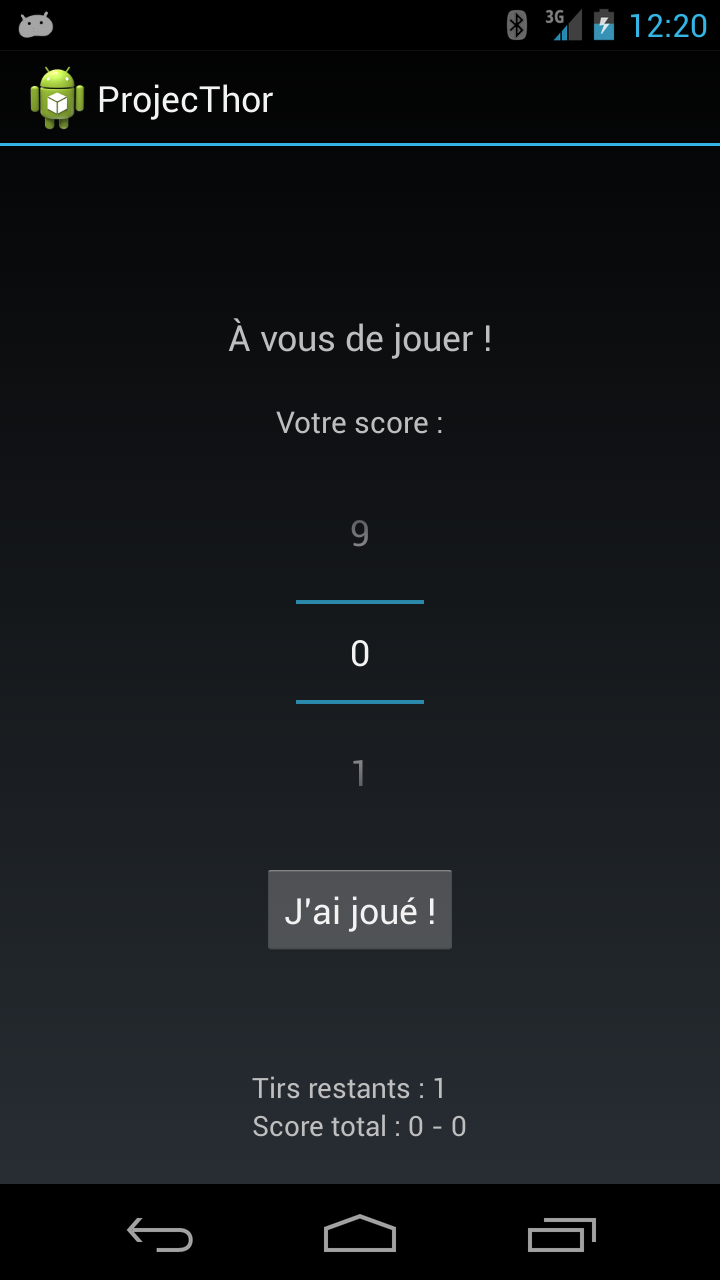
\includegraphics[scale=0.2]{view_3.png}
	\end{minipage}

\end{figure}

\begin{figure}

	\begin{minipage}{0.45\textwidth}
		\caption{Chargement du canon}
		\label{view_4}
		\center
		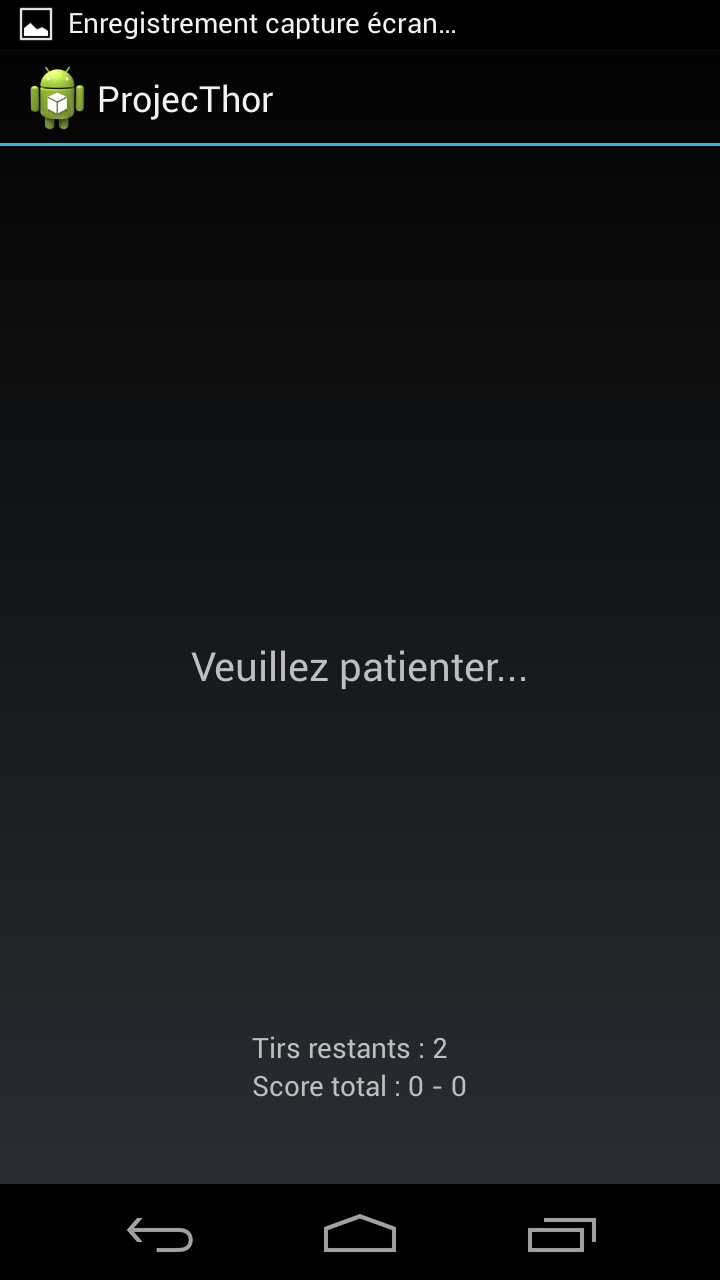
\includegraphics[scale=0.2]{view_4.png}
	\end{minipage}
	\hspace{0.1\textwidth}
	\begin{minipage}{0.45\textwidth}
		\caption{Tir du robot}
		\label{view_5}
		\center
		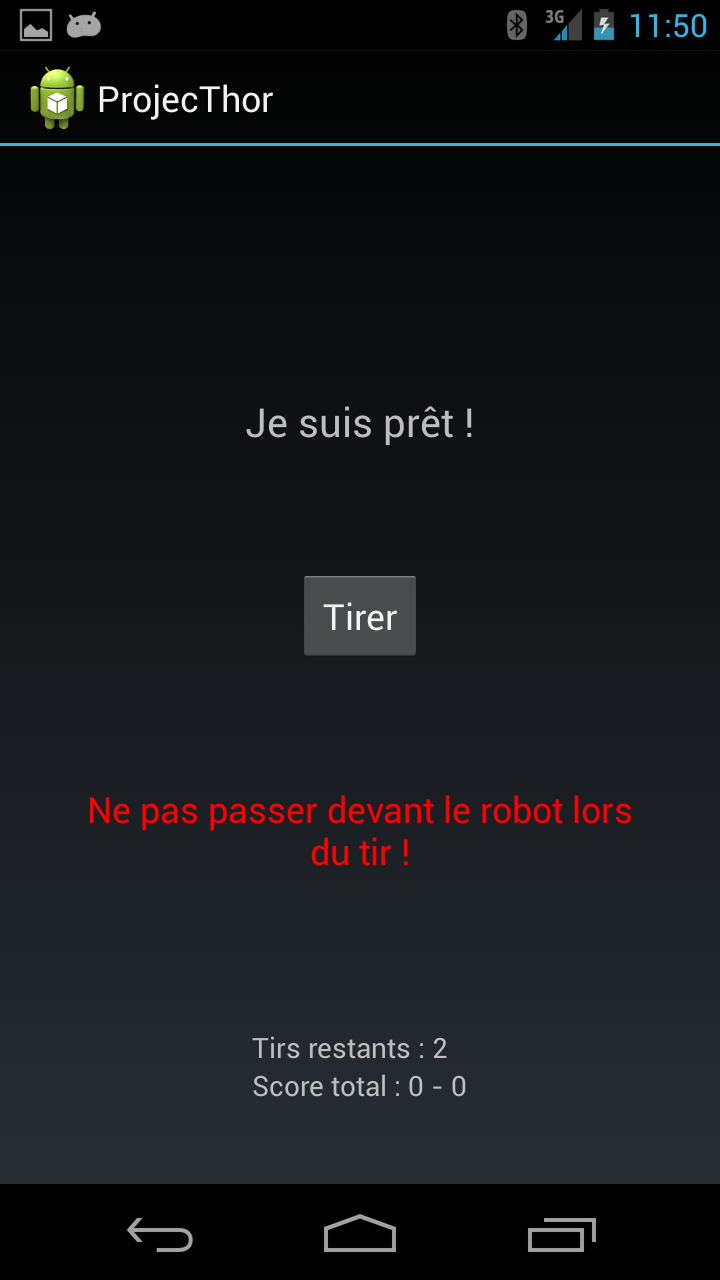
\includegraphics[scale=0.2]{view_5.png}
	\end{minipage}

	\vspace*{20mm}

	\begin{minipage}{0.45\textwidth}
		\caption{Game Over}
		\label{view_6}
		\center
		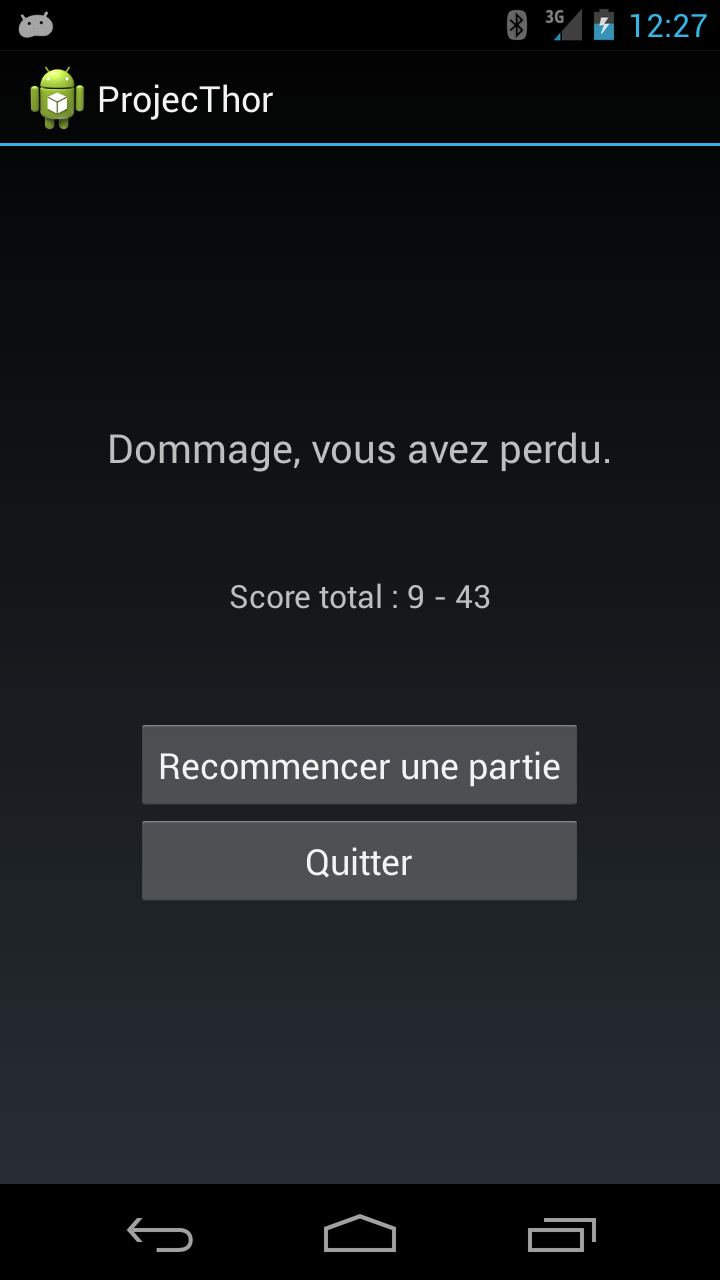
\includegraphics[scale=0.2]{view_6.png}
	\end{minipage}

\end{figure}

\section{Explication du code}

L'application Android est compilée à partir de deux types de fichiers :
\begin{itemize}
	\item Les fichiers sources .java qui décrivent le fonctionnement de l'application à l'aide du langage de programmation Java et des outils de développement Android fournis par Google ; un fichier correspond à une activité (ici il n'y en a qu'une seule : l'activité principale MainActivity)
	\item Les fichiers XML qui décrivent l'interface graphique ; un fichier .xml correspond à une vue (voir la section~\ref{andr_gui} page~\pageref{andr_gui})
\end{itemize}
Le code complet est accessible dans le dossier "android" du CD, et se situe dans les fichiers src/si/tpe/projecthor/MainActivity.java ainsi que dans les fichier .xml du dossier res/layout/.
Ici seul les principales fonctions du code Java sera explicité, l'intérêt d'expliquer l'organisation des éléments de la GUI entre eux à l'aide d'un code XML étant assez limité.

\lstset{language=Java}

\subsection{La fonction onCreate}

\begin{lstlisting}
public void onCreate(Bundle savedInstanceState) {
	super.onCreate(savedInstanceState);
	setContentView(R.layout.connecting);
	
	connexionState = (TextView)findViewById(R.id.connexionState);
	reconnectButton = (Button)findViewById(R.id.reconnectButton);

	bluetoothAdapter = BluetoothAdapter.getDefaultAdapter();
	if(!bluetoothAdapter.isEnabled()) {
		bluetoothAdapter.enable();
		while(!bluetoothAdapter.isEnabled()) { }
	}

	launchConnexion();
}
\end{lstlisting}
Fonction lancée au démarrage de l'application, qui affiche la 1ère vue (fig.~\ref{view_1}) et lance une tentative de connexion avec la fonction launchConnexion. \\

\subsection{La fonction launchConnexion}

\begin{lstlisting}
public void launchConnexion() {
	Set<BluetoothDevice> pairedDevices = bluetoothAdapter.getBondedDevices();
	for(BluetoothDevice device : pairedDevices) {
		if(device.getName().equals(DEVICE_NAME)) {
			connexionState.setText("Connexion en cours...");
			connectThread = new ConnectThread(device);
			connectThread.start();
		}
	}
}
\end{lstlisting}
Cette fonction permet de démarrer la tentative de connexion avec la carte Arduino en lançant le processus de connexion connectThread. Elle est appelée au démarrage de l'application et lors de l'appui sur le bouton "Réessayer" (fig.~\ref{view_0}). \\

\subsection{La fonction handleMessage}

\begin{lstlisting}
\end{lstlisting}
Elles permet de gérer plusieurs cas, selon le message reçu en paramètre :
\begin{itemize}
	\item SUCCEEDED : la connexion avec la carte Arduino a réussi, on affiche donc la deuxième vue (fig.~\ref{view_2})
	\item FAILED : la connexion avec la carte Arduino a échoué, on affiche la vue "Connexion échouée" (fig~\ref{view_0})
	\item MESSAGE\_READ : l'appareil reçoit une information de la part du robot : si le message est la lettre "r", cela indique qu'il est prêt à tirer et et que l'on peut afficher la cinquième vue (fig.~\ref{view_5}) ; sinon c'est qu'il envoie le score qu'il a effectué, que l'on rajoute aux scores précédents pour obtenir à la fin de la partie le score final. C'est aussi ici que l'application détermine si le nombre de manches restantes est nul, auquel cas on génère l'affichage de la sixième vue (fig.~\ref{view_6}) ; on recommence le processus à partir de la troisième vue (fig.~\ref{view_3}) si il reste des manches
\end{itemize}

\subsection{Les fonctions callback}

Elles sont appelées lors de l'appui sur un bouton.

\paragraph{reconnect}

\begin{lstlisting}
public void reconnect(View view) {
	reconnectButton.setVisibility(View.GONE);
	connexionState.setText("Connexion en cours...");
	launchConnexion();
}
\end{lstlisting}
Callback du bouton "Réessayer", qui réaffiche la première vue et relance une tentative de connexion avec la fonction launchConnexion.

\paragraph{launchGame}

\begin{lstlisting}
public void launchGame(View view) {
	connectedThread.write(String.valueOf(difficultyID));
	remainingShots = shotsNumberPicker.getValue();
	displayPlayerRound();
}
\end{lstlisting}
Callback du bouton "C'est parti !", qui affiche la troisième vue et envoie le niveau de difficulté choisi par le joueur à la carte Arduino.

\paragraph{played}

\begin{lstlisting}
public void played(View view) {
	remainingShots--;
	playerScore += playerScoreNumberPicker.getValue();

	setContentView(R.layout.robot_loading);
	refreshScore();

	connectedThread.write("c");
}
\end{lstlisting}
Callback du bouton "J'ai joué !" qui additionne le score entré par le joueur à son score total, décrémente la variable contenant le nombre de manches, envoie l'ordre de préparer le canon à tirer au robot puis affiche la quatrième vue (fig.~\ref{view_4}).

\paragraph{fire}

\begin{lstlisting}
public void fire(View view) {
	connectedThread.write("f");
}
\end{lstlisting}
Callback du bouton "Tirer" qui envoie l'ordre de tirer au robot.

\paragraph{replay}

\begin{lstlisting}
public void replay(View view) {
	displayMain();
	remainingShots = 3;
	playerScore = 0;
	robotScore = 0;
}
\end{lstlisting}
Callback du bouton "Recommencer une partie" qui repart à la deuxième vue et remet les scores et le nombre de manches restantes à 0.

\paragraph{quit}

\begin{lstlisting}
public void quit(View view) {
	connectThread.cancel();
	connectedThread.cancel();
	finish();
}
\end{lstlisting}
Callback du bouton "Quitter" qui coupe la connexion avec la carte et quitte l'application.

